\documentclass[aspectratio=169,11pt]{beamer}

% TEMA Y COLORES
\usetheme{Madrid}
\usecolortheme{whale}

\definecolor{primaryblue}{RGB}{0,102,153}
\definecolor{accentgreen}{RGB}{0,128,0}
\definecolor{accentorange}{RGB}{204,102,0}
\definecolor{darkgray}{RGB}{64,64,64}

\setbeamercolor{palette primary}{bg=primaryblue,fg=white}
\setbeamercolor{palette secondary}{bg=primaryblue!80,fg=white}
\setbeamercolor{palette tertiary}{bg=primaryblue!60,fg=white}
\setbeamercolor{structure}{fg=primaryblue}
\setbeamercolor{block title}{bg=primaryblue,fg=white}
\setbeamercolor{block body}{bg=primaryblue!10}
\setbeamercolor{block title example}{bg=accentgreen,fg=white}
\setbeamercolor{block body example}{bg=accentgreen!10}
\setbeamercolor{block title alerted}{bg=accentorange,fg=white}
\setbeamercolor{block body alerted}{bg=accentorange!10}

% PAQUETES
\usepackage[utf8]{inputenc}
\usepackage[T1]{fontenc}
\usepackage{amsmath,amssymb}
\usepackage{booktabs}
\usepackage{tikz}
\usepackage{pgfplots}
\usepackage{listings}
\usepackage{multicol}

\pgfplotsset{compat=1.17}

% CÓDIGO PYTHON
\lstdefinestyle{pythonstyle}{
    language=Python,
    basicstyle=\ttfamily\footnotesize,
    keywordstyle=\color{blue}\bfseries,
    stringstyle=\color{red},
    commentstyle=\color{accentgreen}\itshape,
    frame=single,
    breaklines=true,
    showstringspaces=false,
    backgroundcolor=\color{gray!10}
}

% NAVEGACIÓN Y PIE DE PÁGINA
\setbeamertemplate{navigation symbols}{}
\setbeamertemplate{footline}{
    \leavevmode%
    \hbox{%
        \begin{beamercolorbox}[wd=.333333\paperwidth,ht=2.25ex,dp=1ex,center]{author in head/foot}%
            \usebeamerfont{author in head/foot}Matemáticas Financieras
        \end{beamercolorbox}%
        \begin{beamercolorbox}[wd=.333333\paperwidth,ht=2.25ex,dp=1ex,center]{title in head/foot}%
            \usebeamerfont{title in head/foot}Sesión 3
        \end{beamercolorbox}%
        \begin{beamercolorbox}[wd=.333333\paperwidth,ht=2.25ex,dp=1ex,right]{date in head/foot}%
            \usebeamerfont{date in head/foot}\insertframenumber{} / \inserttotalframenumber\hspace*{2ex}
        \end{beamercolorbox}}%
    \vskip0pt%
}

\title[Sesión 3]{Tasas Nominales, Efectivas y Equivalentes}
\subtitle{Entendiendo la verdadera tasa de interés}
\author{Matemáticas Financieras}
\institute{Valor del Dinero en el Tiempo}
\date{Semana 2 | Clase 1 | Duración: 1h 50min}

\begin{document}

% ===========================================
% SECCIÓN 1: PORTADA Y CONTENIDO
% ===========================================

\begin{frame}
    \titlepage
\end{frame}

\begin{frame}{Contenido de la Sesión}
    \tableofcontents
\end{frame}

% ===========================================
% SECCIÓN 2: INTRODUCCIÓN
% ===========================================
\section{Introducción}

\begin{frame}{Conexión con la Sesión Anterior}
    \begin{block}{Sesiones 1 y 2: Capitalización y Descuento}
        Aprendimos a calcular VP y VF usando una tasa $r$ por período:
        \[
        F = P(1 + r)^n \quad \text{y} \quad P = \frac{F}{(1 + r)^n}
        \]
    \end{block}

    \pause
    \vspace{0.3cm}

    \begin{alertblock}{Pero surge una pregunta...}
        ¿Qué pasa cuando la capitalización \textbf{no es anual}?

        \vspace{0.2cm}
        \textit{``El banco ofrece 12\% anual con capitalización mensual...''}

        \vspace{0.2cm}
        ¿Es lo mismo que 12\% anual con capitalización anual?
    \end{alertblock}
\end{frame}

\begin{frame}{Objetivos de Aprendizaje}
    Al finalizar esta sesión, serás capaz de:
    \begin{enumerate}
        \item Distinguir entre tasa nominal y tasa efectiva
        \item Calcular la tasa efectiva dada cualquier frecuencia de capitalización
        \item Convertir entre tasas con diferentes períodos de capitalización
        \item Comprender y aplicar la tasa de interés continua
        \item Diferenciar entre APR y APY (y su uso en la práctica)
        \item Entender puntos base y puntos porcentuales
    \end{enumerate}
\end{frame}

\begin{frame}{Motivación: Comparando Ofertas Bancarias}
    \begin{block}{Escenario}
        Tres bancos ofrecen cuentas de ahorro:
        \begin{itemize}
            \item \textbf{Banco A:} 12\% anual, capitalización anual
            \item \textbf{Banco B:} 12\% anual, capitalización mensual
            \item \textbf{Banco C:} 11.9\% anual, capitalización diaria
        \end{itemize}

        ¿Cuál es la mejor opción?
    \end{block}

    \pause
    \vspace{0.5cm}

    \begin{exampleblock}{Spoiler}
        Todas reportan tasas similares, pero el \textbf{rendimiento real} es diferente. Necesitamos herramientas para compararlas correctamente.
    \end{exampleblock}
\end{frame}

% ===========================================
% SECCIÓN 3: DERIVACIONES MATEMÁTICAS
% ===========================================
\section{Tasa Nominal vs. Efectiva}

\begin{frame}{Definiciones Fundamentales}
    \begin{block}{Tasa Nominal ($r_{nom}$)}
        Tasa de interés \textbf{anunciada} o cotizada, que no refleja el efecto de la capitalización. También llamada APR (Annual Percentage Rate).
    \end{block}

    \pause
    \vspace{0.3cm}

    \begin{block}{Tasa Efectiva ($r_{ef}$)}
        Tasa de interés que \textbf{realmente} se gana o paga en un año, considerando el efecto de la capitalización. También llamada APY (Annual Percentage Yield) o EAR (Effective Annual Rate).
    \end{block}

    \pause
    \vspace{0.3cm}

    \begin{block}{Frecuencia de Capitalización ($m$)}
        Número de veces por año que se calculan y acumulan los intereses.
    \end{block}
\end{frame}

\begin{frame}{Capitalización $m$ veces al año}
    Si la tasa nominal es $r_{nom}$ y se capitaliza $m$ veces al año:

    \pause
    \vspace{0.3cm}

    \textbf{Tasa por período de capitalización:}
    \[
    r_{\text{período}} = \frac{r_{nom}}{m}
    \]

    \pause
    \vspace{0.3cm}

    \textbf{Número de períodos en un año:}
    \[
    \text{Períodos por año} = m
    \]

    \pause
    \vspace{0.3cm}

    \textbf{Valor futuro después de 1 año:}
    \[
    F = P\left(1 + \frac{r_{nom}}{m}\right)^m
    \]
\end{frame}

\begin{frame}{Derivación de la Tasa Efectiva}
    La tasa efectiva es aquella que, aplicada una sola vez al año, produce el mismo valor futuro.

    \pause
    \vspace{0.3cm}

    \textbf{Con capitalización $m$ veces:}
    \[
    F = P\left(1 + \frac{r_{nom}}{m}\right)^m
    \]

    \pause
    \textbf{Con tasa efectiva (capitalización anual):}
    \[
    F = P(1 + r_{ef})
    \]

    \pause
    \textbf{Igualando:}
    \begin{align*}
        P(1 + r_{ef}) &= P\left(1 + \frac{r_{nom}}{m}\right)^m \\
        1 + r_{ef} &= \left(1 + \frac{r_{nom}}{m}\right)^m
    \end{align*}
\end{frame}

\begin{frame}{Fórmula de la Tasa Efectiva}
    \begin{block}{Tasa Efectiva Anual}
        \[
        \boxed{r_{ef} = \left(1 + \frac{r_{nom}}{m}\right)^m - 1}
        \]
    \end{block}

    \pause
    \vspace{0.5cm}

    \textbf{Frecuencias comunes de capitalización:}
    \begin{center}
    \begin{tabular}{@{}lc@{}}
        \toprule
        \textbf{Frecuencia} & $m$ \\
        \midrule
        Anual & 1 \\
        Semestral & 2 \\
        Trimestral & 4 \\
        Mensual & 12 \\
        Semanal & 52 \\
        Diaria & 365 \\
        \bottomrule
    \end{tabular}
    \end{center}
\end{frame}

\begin{frame}{Ejemplo: Calculando la Tasa Efectiva}
    \begin{block}{Problema}
        Un banco ofrece 12\% nominal anual con capitalización mensual. ¿Cuál es la tasa efectiva anual?
    \end{block}

    \pause
    \vspace{0.3cm}

    \textbf{Datos:}
    \begin{itemize}
        \item $r_{nom} = 0.12$ (12\%)
        \item $m = 12$ (mensual)
    \end{itemize}

    \pause
    \vspace{0.3cm}

    \textbf{Cálculo:}
    \begin{align*}
        r_{ef} &= \left(1 + \frac{0.12}{12}\right)^{12} - 1 \\
        r_{ef} &= (1 + 0.01)^{12} - 1 \\
        r_{ef} &= (1.01)^{12} - 1 \\
        r_{ef} &= 1.1268 - 1 = 0.1268 = 12.68\%
    \end{align*}
\end{frame}

\begin{frame}{Efecto de la Frecuencia de Capitalización}
    \textbf{12\% nominal anual con diferentes capitalizaciones:}

    \vspace{0.3cm}

    \begin{center}
    \begin{tabular}{@{}lccl@{}}
        \toprule
        \textbf{Capitalización} & $m$ & $(1 + 0.12/m)^m$ & $r_{ef}$ \\
        \midrule
        Anual & 1 & 1.1200 & 12.00\% \\
        Semestral & 2 & 1.1236 & 12.36\% \\
        Trimestral & 4 & 1.1255 & 12.55\% \\
        Mensual & 12 & 1.1268 & 12.68\% \\
        Semanal & 52 & 1.1273 & 12.73\% \\
        Diaria & 365 & 1.1275 & 12.75\% \\
        Continua & $\infty$ & $e^{0.12}$ & 12.75\% \\
        \bottomrule
    \end{tabular}
    \end{center}

    \pause
    \vspace{0.3cm}

    \begin{alertblock}{Observación}
        A mayor frecuencia de capitalización, mayor tasa efectiva. Pero converge a un límite.
    \end{alertblock}
\end{frame}

\section{Tasa de Interés Continua}

\begin{frame}{Capitalización Continua: Derivación}
    ¿Qué pasa cuando $m \to \infty$?

    \pause
    \vspace{0.3cm}

    Recordemos el límite fundamental:
    \[
    \lim_{n \to \infty} \left(1 + \frac{1}{n}\right)^n = e \approx 2.71828
    \]

    \pause
    \vspace{0.3cm}

    Aplicando a nuestra fórmula:
    \begin{align*}
        \lim_{m \to \infty} \left(1 + \frac{r_{nom}}{m}\right)^m &= e^{r_{nom}}
    \end{align*}

    \pause
    \vspace{0.3cm}

    \begin{block}{Valor Futuro con Capitalización Continua}
        \[
        \boxed{F = P \cdot e^{r \cdot t}}
        \]
        donde $r$ es la tasa continua y $t$ es el tiempo en años.
    \end{block}
\end{frame}

\begin{frame}{Conversión entre Tasa Continua y Efectiva}
    \textbf{De continua a efectiva:}
    \[
    \boxed{r_{ef} = e^{r_c} - 1}
    \]

    \pause
    \vspace{0.5cm}

    \textbf{De efectiva a continua:}
    \[
    \boxed{r_c = \ln(1 + r_{ef})}
    \]

    \pause
    \vspace{0.5cm}

    \begin{exampleblock}{Ejemplo}
        Si $r_c = 10\%$ continuo:
        \[
        r_{ef} = e^{0.10} - 1 = 1.1052 - 1 = 10.52\%
        \]
    \end{exampleblock}
\end{frame}

\begin{frame}{¿Por qué usar Tasas Continuas?}
    \begin{block}{Ventajas Matemáticas}
        \begin{itemize}
            \item Simplifica derivadas e integrales
            \item Las tasas continuas son \textbf{aditivas} en el tiempo
            \item Fundamental en modelos de opciones (Black-Scholes)
            \item Facilita el cálculo de rendimientos logarítmicos
        \end{itemize}
    \end{block}

    \pause
    \vspace{0.5cm}

    \begin{exampleblock}{Aditividad de Tasas Continuas}
        Si inviertes al 5\% continuo por 2 años y luego al 8\% continuo por 3 años:
        \[
        F = P \cdot e^{0.05 \times 2} \cdot e^{0.08 \times 3} = P \cdot e^{0.10 + 0.24} = P \cdot e^{0.34}
        \]
    \end{exampleblock}
\end{frame}

\section{Conversión entre Tasas}

\begin{frame}{Tasas Equivalentes}
    \begin{block}{Definición}
        Dos tasas son \textbf{equivalentes} si producen el mismo valor futuro en el mismo período de tiempo, independientemente de la frecuencia de capitalización.
    \end{block}

    \pause
    \vspace{0.5cm}

    \textbf{Fórmula de equivalencia:}
    \[
    \boxed{\left(1 + \frac{r_1}{m_1}\right)^{m_1} = \left(1 + \frac{r_2}{m_2}\right)^{m_2}}
    \]

    \pause
    \vspace{0.3cm}

    Para encontrar $r_2$ dado $r_1$:
    \[
    r_2 = m_2 \left[\left(1 + \frac{r_1}{m_1}\right)^{m_1/m_2} - 1\right]
    \]
\end{frame}

\begin{frame}{Ejemplo: Convertir Tasas}
    \begin{block}{Problema}
        Un préstamo cobra 18\% nominal anual con capitalización mensual. ¿Cuál es la tasa trimestral equivalente?
    \end{block}

    \pause
    \vspace{0.3cm}

    \textbf{Paso 1:} Calcular tasa efectiva anual
    \begin{align*}
        r_{ef} = \left(1 + \frac{0.18}{12}\right)^{12} - 1 = (1.015)^{12} - 1 = 19.56\%
    \end{align*}

    \pause
    \textbf{Paso 2:} Convertir a tasa trimestral
    \begin{align*}
        1 + r_{ef} &= (1 + r_T)^4 \\
        1.1956 &= (1 + r_T)^4 \\
        r_T &= (1.1956)^{1/4} - 1 = 0.0456 = 4.56\%
    \end{align*}

    \pause
    \textbf{Tasa nominal trimestral:} $4.56\% \times 4 = 18.24\%$ anual capitalizable trimestralmente.
\end{frame}

\begin{frame}{APR vs. APY}
    \begin{columns}
        \begin{column}{0.48\textwidth}
            \begin{block}{APR (Annual Percentage Rate)}
                \begin{itemize}
                    \item Tasa nominal anual
                    \item \textbf{No} incluye efecto de capitalización
                    \item Usada para \textbf{préstamos}
                    \item Subestima el costo real
                \end{itemize}
            \end{block}
        \end{column}

        \begin{column}{0.48\textwidth}
            \begin{block}{APY (Annual Percentage Yield)}
                \begin{itemize}
                    \item Tasa efectiva anual
                    \item \textbf{Sí} incluye capitalización
                    \item Usada para \textbf{ahorros}
                    \item Refleja el rendimiento real
                \end{itemize}
            \end{block}
        \end{column}
    \end{columns}

    \pause
    \vspace{0.5cm}

    \begin{alertblock}{Regla práctica en EE.UU.}
        \begin{itemize}
            \item Bancos \textbf{anuncian APY} en cuentas de ahorro (parece mejor)
            \item Bancos \textbf{anuncian APR} en préstamos (parece menor)
            \item ¡Siempre compara usando la misma métrica!
        \end{itemize}
    \end{alertblock}
\end{frame}

\section{Puntos Base y Porcentuales}

\begin{frame}{Puntos Porcentuales vs. Puntos Base}
    \begin{block}{Punto Porcentual (pp)}
        Diferencia aritmética entre dos porcentajes.

        \textbf{Ejemplo:} Si la tasa sube de 5\% a 7\%, subió \textbf{2 puntos porcentuales}.
    \end{block}

    \pause
    \vspace{0.3cm}

    \begin{block}{Punto Base (pb o bp)}
        Una centésima de punto porcentual.
        \[
        \boxed{1 \text{ punto base} = 0.01\% = 0.0001}
        \]
        \[
        \boxed{100 \text{ puntos base} = 1\%}
        \]
    \end{block}

    \pause
    \vspace{0.3cm}

    \begin{exampleblock}{Ejemplo}
        Si la tasa sube de 5.25\% a 5.50\%, subió \textbf{25 puntos base} (o 0.25 pp).
    \end{exampleblock}
\end{frame}

\begin{frame}{¿Por qué usar Puntos Base?}
    \begin{alertblock}{Evita ambigüedad}
        ``La tasa subió 10\%'' puede significar:
        \begin{itemize}
            \item De 5\% a 15\% (subió 10 puntos porcentuales)
            \item De 5\% a 5.5\% (subió 10\% relativo, o 50 pb)
        \end{itemize}

        ``La tasa subió 50 puntos base'' es inequívoco: de 5\% a 5.50\%.
    \end{alertblock}

    \pause
    \vspace{0.5cm}

    \textbf{Uso común en finanzas:}
    \begin{itemize}
        \item Bancos centrales: ``El Fed subió la tasa 25 pb''
        \item Spreads de crédito: ``El spread es de 150 pb sobre LIBOR''
        \item Comisiones: ``El fondo cobra 75 pb anuales''
    \end{itemize}
\end{frame}

\begin{frame}{Conversiones Rápidas}
    \begin{center}
    \begin{tabular}{@{}ccc@{}}
        \toprule
        \textbf{Puntos Base} & \textbf{Puntos Porcentuales} & \textbf{Decimal} \\
        \midrule
        1 bp & 0.01\% & 0.0001 \\
        10 bp & 0.10\% & 0.0010 \\
        25 bp & 0.25\% & 0.0025 \\
        50 bp & 0.50\% & 0.0050 \\
        100 bp & 1.00\% & 0.0100 \\
        150 bp & 1.50\% & 0.0150 \\
        \bottomrule
    \end{tabular}
    \end{center}

    \pause
    \vspace{0.5cm}

    \begin{exampleblock}{Ejemplo de impacto}
        En un préstamo de \$1,000,000, un aumento de 25 pb significa:
        \[
        \$1,000,000 \times 0.0025 = \$2,500 \text{ adicionales por año}
        \]
    \end{exampleblock}
\end{frame}

% ===========================================
% SECCIÓN 4: INTERPRETACIÓN VISUAL
% ===========================================
\section{Interpretación Visual}

\begin{frame}{Gráfica: Tasa Efectiva vs. Frecuencia}
    \begin{center}
        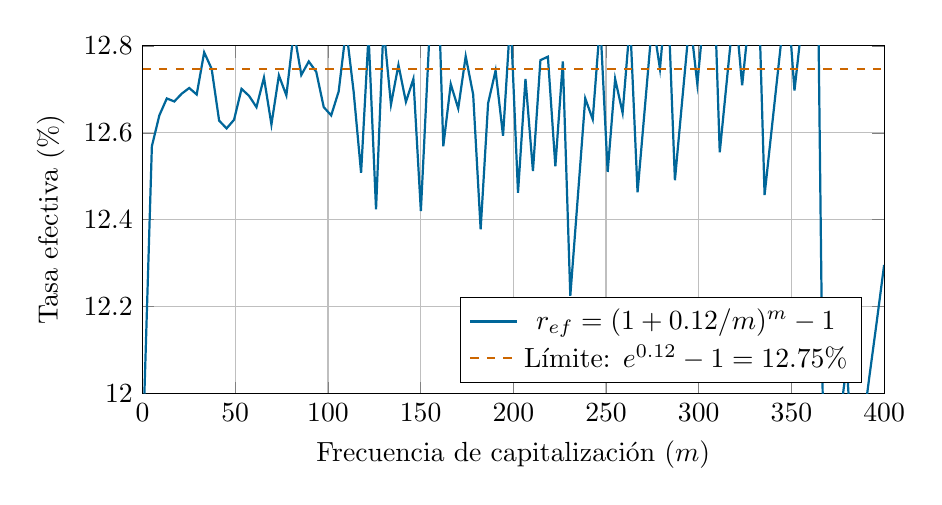
\begin{tikzpicture}
            \begin{axis}[
                xlabel={Frecuencia de capitalización ($m$)},
                ylabel={Tasa efectiva (\%)},
                xmin=0, xmax=400,
                ymin=12, ymax=12.8,
                grid=major,
                width=11cm,
                height=6cm,
                legend pos=south east
            ]
            % Tasa efectiva
            \addplot[color=primaryblue, thick, domain=1:400, samples=100] {((1+0.12/x)^x - 1)*100};
            \addlegendentry{$r_{ef} = (1+0.12/m)^m - 1$}
            % Límite continuo
            \addplot[color=accentorange, thick, dashed, domain=0:400] {(2.71828^0.12 - 1)*100};
            \addlegendentry{Límite: $e^{0.12}-1 = 12.75\%$}
            \end{axis}
        \end{tikzpicture}
    \end{center}

    \textbf{Observación:} La tasa efectiva converge rápidamente al límite continuo.
\end{frame}

\begin{frame}{Comparación Visual: Capitalización}
    \textbf{Crecimiento de \$1,000 al 12\% nominal por 5 años:}

    \begin{center}
        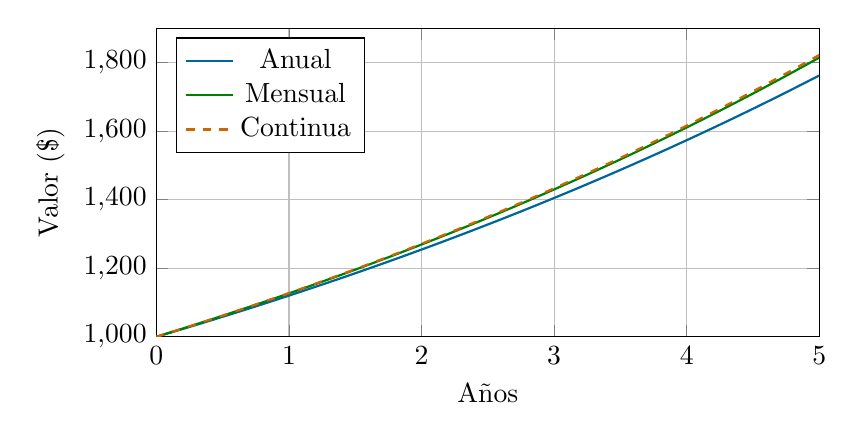
\begin{tikzpicture}
            \begin{axis}[
                xlabel={Años},
                ylabel={Valor (\$)},
                xmin=0, xmax=5,
                ymin=1000, ymax=1900,
                grid=major,
                width=10cm,
                height=5.5cm,
                legend pos=north west
            ]
            % Anual
            \addplot[color=primaryblue, thick, domain=0:5, samples=50] {1000*(1.12)^x};
            \addlegendentry{Anual}
            % Mensual
            \addplot[color=accentgreen, thick, domain=0:5, samples=50] {1000*(1+0.12/12)^(12*x)};
            \addlegendentry{Mensual}
            % Continua
            \addplot[color=accentorange, thick, dashed, domain=0:5, samples=50] {1000*exp(0.12*x)};
            \addlegendentry{Continua}
            \end{axis}
        \end{tikzpicture}
    \end{center}
\end{frame}

% ===========================================
% SECCIÓN 5: TRUCOS DE ESTIMACIÓN
% ===========================================
\section{Trucos de Estimación Mental}

\begin{frame}{Aproximación para Tasas Pequeñas}
    \begin{alertblock}{Aproximación de Taylor}
        Para $r$ pequeño y $m$ grande:
        \[
        \left(1 + \frac{r}{m}\right)^m \approx 1 + r + \frac{r^2}{2}
        \]
    \end{alertblock}

    \pause
    \vspace{0.3cm}

    \textbf{Implicación:}
    \[
    r_{ef} \approx r_{nom} + \frac{r_{nom}^2}{2}
    \]

    \pause
    \vspace{0.3cm}

    \begin{exampleblock}{Ejemplo}
        Con $r_{nom} = 10\%$:
        \[
        r_{ef} \approx 0.10 + \frac{(0.10)^2}{2} = 0.10 + 0.005 = 10.5\%
        \]
        Exacto con capitalización continua: $e^{0.10} - 1 = 10.52\%$ \checkmark
    \end{exampleblock}
\end{frame}

\begin{frame}{Regla del ``Medio por Ciento''}
    \begin{alertblock}{Regla Práctica}
        Para tasas nominales alrededor del 10\%, la tasa efectiva es aproximadamente \textbf{medio punto porcentual mayor} cuando se capitaliza continuamente.
    \end{alertblock}

    \pause
    \vspace{0.5cm}

    \begin{center}
    \begin{tabular}{@{}ccc@{}}
        \toprule
        $r_{nom}$ & $r_{ef}$ (continua) & Diferencia \\
        \midrule
        6\% & 6.18\% & +0.18 pp \\
        8\% & 8.33\% & +0.33 pp \\
        10\% & 10.52\% & +0.52 pp \\
        12\% & 12.75\% & +0.75 pp \\
        15\% & 16.18\% & +1.18 pp \\
        \bottomrule
    \end{tabular}
    \end{center}
\end{frame}

\begin{frame}{De Mensual a Anual Rápido}
    \begin{alertblock}{Aproximación Útil}
        Si conoces la tasa mensual $r_m$, la tasa efectiva anual es aproximadamente:
        \[
        r_{ef} \approx 12 \cdot r_m + 66 \cdot r_m^2
        \]
    \end{alertblock}

    \pause
    \vspace{0.3cm}

    \begin{exampleblock}{Ejemplo}
        Tasa mensual de 1\% ($r_m = 0.01$):
        \begin{align*}
            r_{ef} &\approx 12(0.01) + 66(0.01)^2 \\
            &= 0.12 + 0.0066 \\
            &= 12.66\%
        \end{align*}
        Exacto: $(1.01)^{12} - 1 = 12.68\%$ \checkmark
    \end{exampleblock}
\end{frame}

% ===========================================
% SECCIÓN 6: HP 12C
% ===========================================
\section{Calculadora HP 12C}

\begin{frame}{HP 12C: Conversión de Tasas}
    La HP 12C puede convertir entre tasas nominal y efectiva.

    \vspace{0.3cm}

    \begin{center}
    \begin{tabular}{@{}cl@{}}
        \toprule
        \textbf{Teclas} & \textbf{Función} \\
        \midrule
        \texttt{n} & Períodos de capitalización por año ($m$) \\
        \texttt{i} & Tasa nominal anual / períodos \\
        \texttt{PV} & -1 (valor inicial) \\
        \texttt{PMT} & 0 (sin pagos) \\
        \texttt{FV} & Calcula el factor $(1+r/m)^m$ \\
        \bottomrule
    \end{tabular}
    \end{center}

    \pause
    \vspace{0.3cm}

    \textbf{Tasa efectiva = FV - 1} (expresada como decimal).
\end{frame}

\begin{frame}{HP 12C: Ejemplo - Nominal a Efectiva}
    \begin{block}{Problema}
        Convertir 12\% nominal mensual a tasa efectiva anual.
    \end{block}

    \pause
    \vspace{0.3cm}

    \begin{center}
    \begin{tabular}{@{}lll@{}}
        \toprule
        \textbf{Teclas} & \textbf{Display} & \textbf{Descripción} \\
        \midrule
        \texttt{f CLX} & 0.00 & Limpiar \\
        \texttt{12 n} & 12.00 & 12 períodos (mensual) \\
        \texttt{12 ENTER 12 $\div$ i} & 1.00 & Tasa por período (1\%) \\
        \texttt{1 CHS PV} & -1.00 & Valor inicial \\
        \texttt{0 PMT} & 0.00 & Sin pagos \\
        \texttt{FV} & \textbf{1.1268} & Factor de capitalización \\
        \bottomrule
    \end{tabular}
    \end{center}

    \pause
    \vspace{0.3cm}

    \textbf{Tasa efectiva:} $1.1268 - 1 = 0.1268 = 12.68\%$
\end{frame}

\begin{frame}{HP 12C: Ejemplo - Comparar Ofertas}
    \begin{block}{Problema}
        Banco A: 11.5\% nominal trimestral. Banco B: 11.3\% nominal mensual. ¿Cuál es mejor?
    \end{block}

    \pause
    \vspace{0.2cm}

    \textbf{Banco A (trimestral, $m = 4$):}
    \begin{center}
    \begin{tabular}{@{}ll@{}}
        \texttt{4 n}, \texttt{11.5 ENTER 4 $\div$ i}, \texttt{1 CHS PV}, \texttt{0 PMT}, \texttt{FV} & $\to$ 1.1199
    \end{tabular}
    \end{center}
    $r_{ef,A} = 11.99\%$

    \pause
    \vspace{0.2cm}

    \textbf{Banco B (mensual, $m = 12$):}
    \begin{center}
    \begin{tabular}{@{}ll@{}}
        \texttt{12 n}, \texttt{11.3 ENTER 12 $\div$ i}, \texttt{1 CHS PV}, \texttt{0 PMT}, \texttt{FV} & $\to$ 1.1191
    \end{tabular}
    \end{center}
    $r_{ef,B} = 11.91\%$

    \pause
    \vspace{0.3cm}

    \textbf{Conclusión:} Banco A es mejor (11.99\% > 11.91\%) a pesar de menor frecuencia.
\end{frame}

% ===========================================
% SECCIÓN 7: EJERCICIOS PRÁCTICOS
% ===========================================
\section{Ejercicios Prácticos}

\begin{frame}{Ejercicio 1: Tasa Efectiva Básica}
    \begin{block}{Problema}
        Una tarjeta de crédito cobra 24\% nominal anual con capitalización mensual. ¿Cuál es la tasa efectiva anual que realmente pagas?
    \end{block}

    \pause
    \vspace{0.3cm}

    \textbf{Solución:}
    \begin{align*}
        r_{ef} &= \left(1 + \frac{0.24}{12}\right)^{12} - 1 \\[0.2cm]
        &= (1 + 0.02)^{12} - 1 \\[0.2cm]
        &= (1.02)^{12} - 1 \\[0.2cm]
        &= 1.2682 - 1 = 26.82\%
    \end{align*}

    \pause
    \textbf{Respuesta:} La tasa efectiva es 26.82\%, casi 3 pp más que la nominal.
\end{frame}

\begin{frame}{Ejercicio 2: Comparación de Inversiones}
    \begin{block}{Problema}
        Opción A: 9\% nominal semestral. Opción B: 8.8\% nominal mensual. ¿Cuál ofrece mejor rendimiento?
    \end{block}

    \pause
    \vspace{0.3cm}

    \textbf{Opción A:}
    \begin{align*}
        r_{ef,A} = \left(1 + \frac{0.09}{2}\right)^{2} - 1 = (1.045)^2 - 1 = 9.20\%
    \end{align*}

    \pause
    \textbf{Opción B:}
    \begin{align*}
        r_{ef,B} = \left(1 + \frac{0.088}{12}\right)^{12} - 1 = (1.00733)^{12} - 1 = 9.16\%
    \end{align*}

    \pause
    \textbf{Respuesta:} Opción A es ligeramente mejor (9.20\% vs 9.16\%).
\end{frame}

\begin{frame}{Ejercicio 3: Tasa Continua}
    \begin{block}{Problema}
        Un banco ofrece 6\% con capitalización continua. ¿Cuánto tendrás después de 5 años si inviertes \$10,000?
    \end{block}

    \pause
    \vspace{0.3cm}

    \textbf{Solución:}
    \begin{align*}
        F &= P \cdot e^{r \cdot t} \\
        F &= 10,000 \cdot e^{0.06 \times 5} \\
        F &= 10,000 \cdot e^{0.30} \\
        F &= 10,000 \times 1.3499 \\
        F &= \$13,498.59
    \end{align*}

    \pause
    \textbf{Tasa efectiva equivalente:} $r_{ef} = e^{0.06} - 1 = 6.18\%$
\end{frame}

\begin{frame}{Ejercicio 4: Encontrar Tasa Nominal}
    \begin{block}{Problema}
        Si quieres obtener una tasa efectiva del 15\% anual, ¿qué tasa nominal necesitas si la capitalización es trimestral?
    \end{block}

    \pause
    \vspace{0.3cm}

    \textbf{Solución:}
    \begin{align*}
        1 + r_{ef} &= \left(1 + \frac{r_{nom}}{4}\right)^4 \\
        1.15 &= \left(1 + \frac{r_{nom}}{4}\right)^4 \\
        (1.15)^{1/4} &= 1 + \frac{r_{nom}}{4} \\
        1.0356 &= 1 + \frac{r_{nom}}{4} \\
        r_{nom} &= 4 \times 0.0356 = 14.23\%
    \end{align*}

    \pause
    \textbf{Respuesta:} Necesitas 14.23\% nominal trimestral.
\end{frame}

\begin{frame}{Ejercicio 5: Puntos Base}
    \begin{block}{Problema}
        Un bono corporativo rinde 150 puntos base sobre la tasa libre de riesgo de 4.5\%. ¿Cuál es el rendimiento del bono? Si la tasa libre de riesgo sube 75 pb, ¿cuál es el nuevo rendimiento?
    \end{block}

    \pause
    \vspace{0.3cm}

    \textbf{Solución:}

    Rendimiento inicial:
    \begin{align*}
        r_{bono} = 4.5\% + 150 \text{ pb} = 4.5\% + 1.5\% = 6.0\%
    \end{align*}

    \pause
    Nueva tasa libre de riesgo:
    \begin{align*}
        r_{lr,nuevo} = 4.5\% + 75 \text{ pb} = 4.5\% + 0.75\% = 5.25\%
    \end{align*}

    \pause
    Nuevo rendimiento del bono (asumiendo spread constante):
    \begin{align*}
        r_{bono,nuevo} = 5.25\% + 1.5\% = 6.75\%
    \end{align*}
\end{frame}

% ===========================================
% SECCIÓN 8: PYTHON
% ===========================================
\section{Python con numpy-financial}

\begin{frame}[fragile]{Python: Convertir Tasas}
    \begin{lstlisting}[style=pythonstyle]
import numpy as np

def nominal_a_efectiva(r_nom, m):
    """Convierte tasa nominal a efectiva."""
    return (1 + r_nom/m)**m - 1

def efectiva_a_nominal(r_ef, m):
    """Convierte tasa efectiva a nominal."""
    return m * ((1 + r_ef)**(1/m) - 1)

def continua_a_efectiva(r_c):
    """Convierte tasa continua a efectiva."""
    return np.exp(r_c) - 1

def efectiva_a_continua(r_ef):
    """Convierte tasa efectiva a continua."""
    return np.log(1 + r_ef)

# Ejemplos
print(f"12% nominal mensual -> {nominal_a_efectiva(0.12, 12)*100:.2f}% efectiva")
print(f"10% efectiva -> {efectiva_a_nominal(0.10, 12)*100:.2f}% nominal mensual")
print(f"8% continua -> {continua_a_efectiva(0.08)*100:.2f}% efectiva")
    \end{lstlisting}
\end{frame}

\begin{frame}[fragile]{Python: Comparación de Ofertas}
    \begin{lstlisting}[style=pythonstyle]
# Comparar ofertas de bancos
ofertas = [
    ("Banco A", 0.12, 1),     # 12% anual
    ("Banco B", 0.12, 2),     # 12% semestral
    ("Banco C", 0.12, 4),     # 12% trimestral
    ("Banco D", 0.12, 12),    # 12% mensual
    ("Banco E", 0.12, 365),   # 12% diaria
]

print("Banco      | Nominal | Freq  | Efectiva")
print("-" * 45)

for nombre, r_nom, m in ofertas:
    r_ef = (1 + r_nom/m)**m - 1
    freq = ["Anual", "Semest", "Trim", "Mensual", "Diaria"]
    print(f"{nombre:10} | {r_nom*100:5.1f}%  | {m:5d} | {r_ef*100:.2f}%")

# Tasa continua como limite
r_continua = np.exp(0.12) - 1
print(f"{'Continua':10} | {12.0:5.1f}%  | {'inf':>5} | {r_continua*100:.2f}%")
    \end{lstlisting}
\end{frame}

\begin{frame}[fragile]{Python: Gráfica de Convergencia}
    \begin{lstlisting}[style=pythonstyle]
import matplotlib.pyplot as plt

r_nom = 0.12
frecuencias = range(1, 366)
tasas_efectivas = [(1 + r_nom/m)**m - 1 for m in frecuencias]
limite_continuo = np.exp(r_nom) - 1

plt.figure(figsize=(10, 6))
plt.plot(frecuencias, [r*100 for r in tasas_efectivas],
         'b-', label='Tasa efectiva')
plt.axhline(y=limite_continuo*100, color='r', linestyle='--',
            label=f'Limite continuo: {limite_continuo*100:.2f}%')
plt.xlabel('Frecuencia de capitalizacion (m)')
plt.ylabel('Tasa efectiva (%)')
plt.title('Convergencia de Tasa Efectiva')
plt.legend()
plt.grid(True)
plt.savefig('convergencia_tasa.png')
    \end{lstlisting}
\end{frame}

% ===========================================
% SECCIÓN 9: RESUMEN Y TAREA
% ===========================================
\section{Resumen y Tarea}

\begin{frame}{Resumen de Fórmulas}
    \begin{columns}
        \begin{column}{0.5\textwidth}
            \textbf{Tasa Efectiva}
            \[
            r_{ef} = \left(1 + \frac{r_{nom}}{m}\right)^m - 1
            \]

            \vspace{0.3cm}

            \textbf{Capitalización Continua}
            \begin{align*}
                F &= P \cdot e^{r \cdot t} \\
                r_{ef} &= e^{r_c} - 1
            \end{align*}
        \end{column}

        \begin{column}{0.5\textwidth}
            \textbf{Tasa Nominal desde Efectiva}
            \[
            r_{nom} = m\left[(1+r_{ef})^{1/m} - 1\right]
            \]

            \vspace{0.3cm}

            \textbf{Puntos Base}
            \begin{align*}
                1 \text{ pb} &= 0.01\% \\
                100 \text{ pb} &= 1\%
            \end{align*}
        \end{column}
    \end{columns}
\end{frame}

\begin{frame}{Conceptos Clave}
    \begin{enumerate}
        \item La \textbf{tasa nominal} no refleja el efecto de capitalización
        \item La \textbf{tasa efectiva} es el rendimiento real anual
        \item Mayor frecuencia de capitalización = mayor tasa efectiva
        \item El límite es la \textbf{capitalización continua}: $e^r$
        \item \textbf{APR} (nominal) vs. \textbf{APY} (efectiva)
        \item \textbf{Puntos base} eliminan ambigüedad: 100 pb = 1\%
        \item Siempre compara inversiones usando la misma métrica
    \end{enumerate}
\end{frame}

\begin{frame}{Tarea para la Próxima Sesión}
    \begin{enumerate}
        \item \textbf{Ejercicios HP 12C:}
        \begin{itemize}
            \item Convertir 18\% nominal mensual a tasa efectiva
            \item Encontrar tasa nominal trimestral equivalente a 10\% efectiva
        \end{itemize}

        \vspace{0.3cm}

        \item \textbf{Problema:} Un préstamo cobra 1.5\% mensual. Calcula (a) APR, (b) APY, (c) cuánto pagarás de interés en un año sobre \$100,000.

        \vspace{0.3cm}

        \item \textbf{Python:} Crea una función que reciba una tasa en cualquier formato (nominal, efectiva, continua) y la convierta a los otros dos.

        \vspace{0.3cm}

        \item \textbf{Reflexión:} ¿Por qué crees que las regulaciones en algunos países exigen que los bancos publiquen la tasa efectiva (APY)?
    \end{enumerate}
\end{frame}

% ===========================================
% CIERRE
% ===========================================

\begin{frame}
    \begin{center}
        \Huge \textcolor{primaryblue}{\textbf{¿Preguntas?}}

        \vspace{1cm}
        \Large Próxima Sesión:\\
        \textbf{Inflación y Tasas Reales}

        \vspace{0.5cm}
        \normalsize Semana 2, Clase 2
    \end{center}
\end{frame}

\end{document}
